\documentclass[11pt]{article}
% \usepackage{lmodern}
%\usepackage[no-math]{fontspec}
%\setmainfont{Arial}

\usepackage[margin=2cm,a4paper]{geometry}
\usepackage{setspace}
\onehalfspacing

\usepackage{graphicx}
\graphicspath{{./fig/}}

\usepackage{wrapfig}
\usepackage[font={small,it}]{caption}
\usepackage[backend=biber,
%style=authoryear,
style=numeric,
giveninits=true,
doi=false,isbn=false,url=false,eprint=false,
natbib,
maxbibnames=10]{biblatex}
\addbibresource[datatype=bibtex]{bibliography.bib}

% % Helper function to get initial letter
% \def\firstinit#1{\justfirst#1\relax}
% \def\justfirst#1#2\relax{#1}

% % Format for FirstInitials - LastName (standard implementation)
% \DeclareNameFormat{firstinits-last}{%
% \usebibmacro{name:first-last}{#1}{#4}{#5}{#7}%
% \usebibmacro{name:andothers}}

% % Format for VeryFirstInitial - LastName
% \DeclareNameFormat{firstfirstinit-last}{%
% \usebibmacro{name:first-last}{#1}{\firstinit{#4}\adddot}{#5}{#7}%
% \usebibmacro{name:andothers}}

% % Set format for sortname (bibliography) and labelname (citation)
% \DeclareNameAlias{sortname}{firstinits-last}
% \DeclareNameAlias{labelname}{firstfirstinit-last}






\usepackage{xcolor}

\usepackage{titlesec}

\titleformat{\section}
  {\normalfont\normalsize\bfseries}{\thesection}{1em}{}
  
\titleformat{\subsection}
  {\normalfont\small\bfseries}{\thesubsection}{1em}{}
  
\usepackage{amsmath}  
\makeatletter
\DeclareRobustCommand{\V}{\text{\volumedash}V}
\newcommand{\volumedash}{%
  \makebox[0pt][l]{%
    \ooalign{\hfil\hphantom{$\m@th V$}\hfil\cr\kern0.08em--\hfil\cr}%
  }%
}
\makeatother

\begin{document}
\rightline{ISF application number: XXX/XX}
\rightline{PI Name: Israel Israeli}

\section*{Research title: fluid dynamics of ideas  }
% up to 10 pages not including figures
\setcounter{section}{0}
\setcounter{subsection}{0}

\section*{Scientific background}

Background 

\setlength{\intextsep}{0pt}%
\begin{wrapfigure}{r}{0.25\textwidth}
    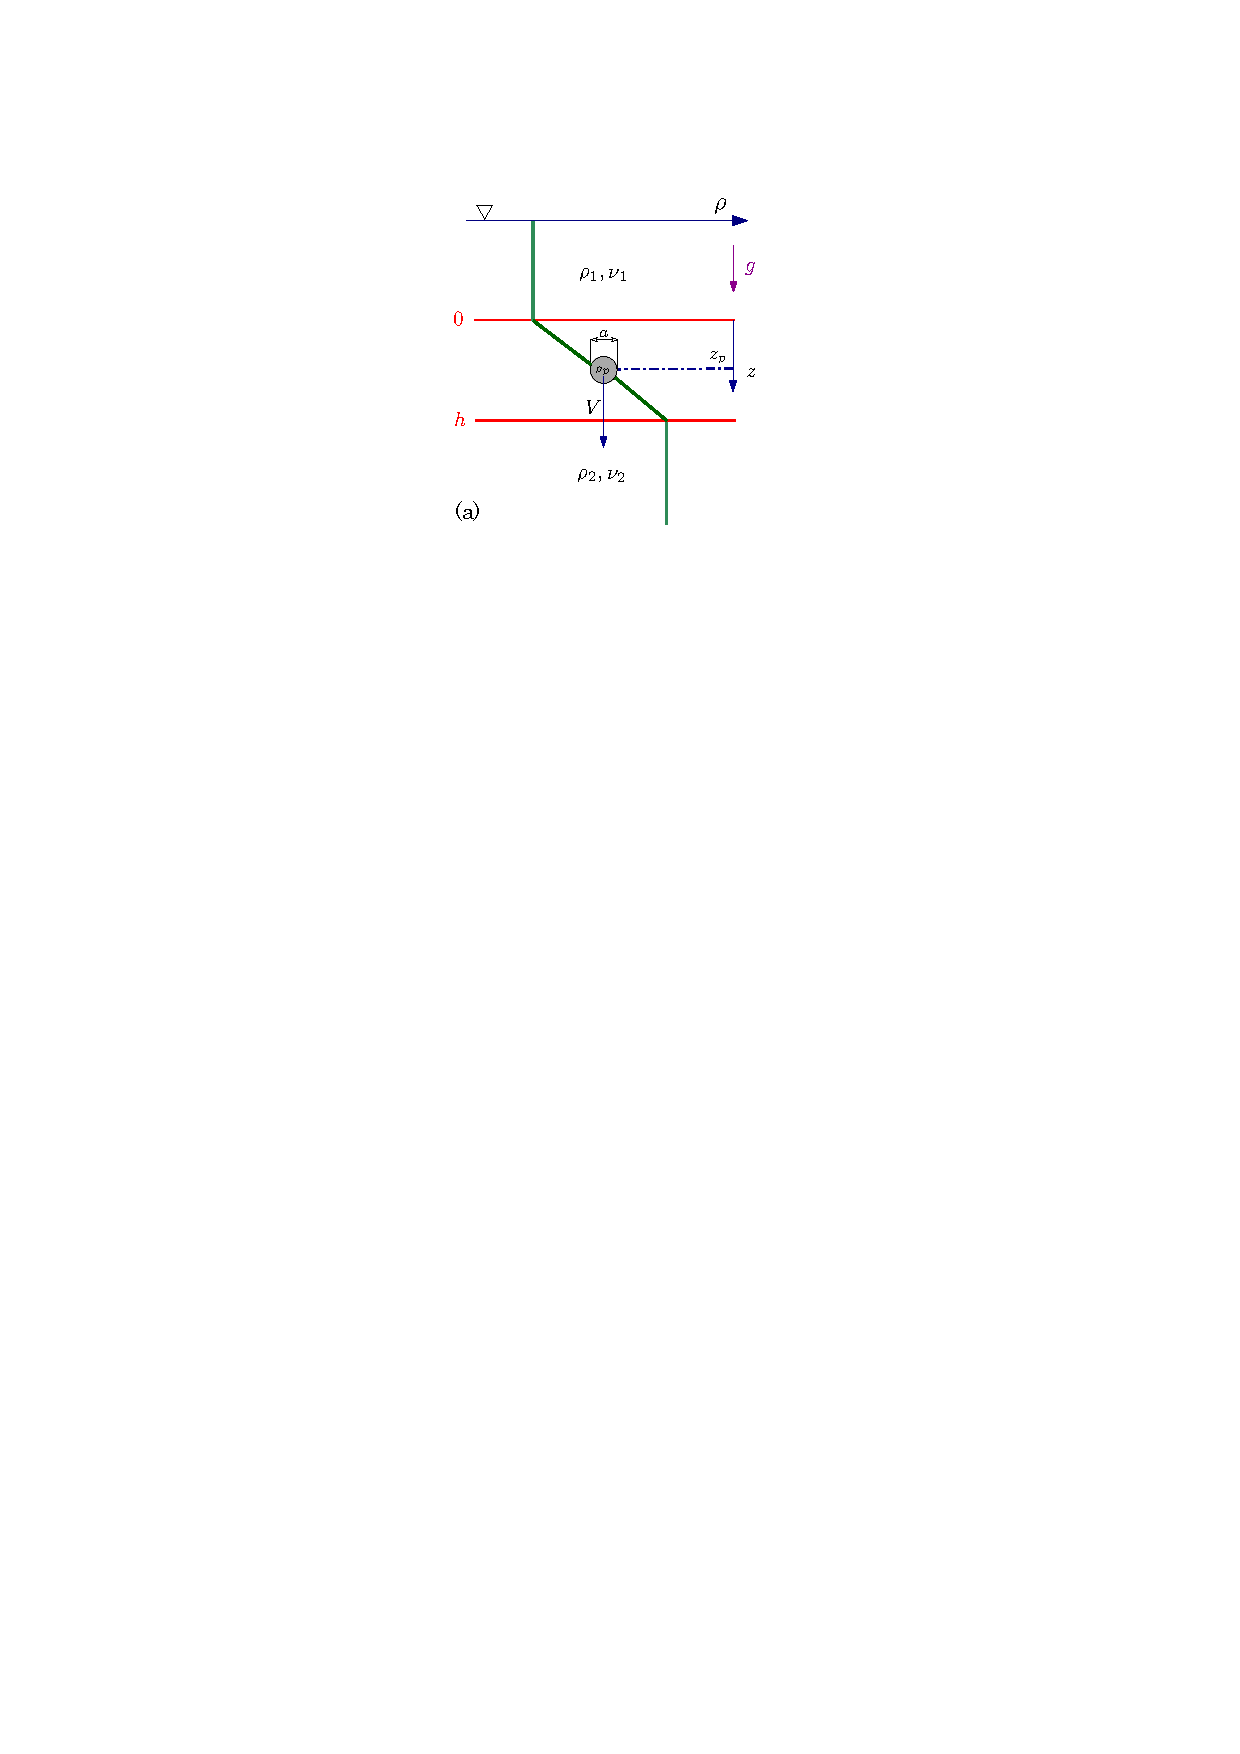
\includegraphics[width=0.23\textwidth]{pdf_fig2}
  \vspace{-10pt}
 \caption{Schematic description of the problem.}
\end{wrapfigure}
%

\subsubsection*{Equations }

\subsection*{Summary}

To sum up, we know a-b-c but do not know d-e-f \cite{dracos1996, Turco1983}

\section*{Research objectives \& expected significance}

This research aims to improve our understanding of the problem 

To achieve this goal, we need to address the following objectives. For the \emph{single particle case}: 
\begin{enumerate}
\item a
\item b
\end{enumerate}


\subsection*{Expected significance}

Of course we're going to change the world

\section*{Detailed research plan}

In details, we are going to measure some stuff and learn from it



\subsection*{Working hypothesis}

This study focuses on ... Our hypothesis is ...
\begin{enumerate}
    \item a
    \item b
    \item c
    \item d
\end{enumerate}


\subsection*{Research design \& methods}

This is our design and these are our methods

\subsection*{Experimental setup}


\subsection*{Data reduction, analysis and modeling plan}


\section*{Preliminary results}



\section*{Existing infrastructure}

We have quite some stuff

\section*{Expected results \& risk management}

We expect some things to change. If a-b-c won't work, we'll do something else
 
\clearpage
%\singlespacing
\printbibliography
\end{document}
